\subsection{Angled crack in an orthotropic body}

\paragraph{}
In this example, consider an orthotropic plate $(b/h = 1)$ with an angled center-crack of length $a/h = 0.5$ under uniform far field tension along the two opposite sides (see fig.~\ref{iso_fig:angled_crack_geo_bc}). 
    \begin{figure}
        \centering
        \scalebox{0.5}{
            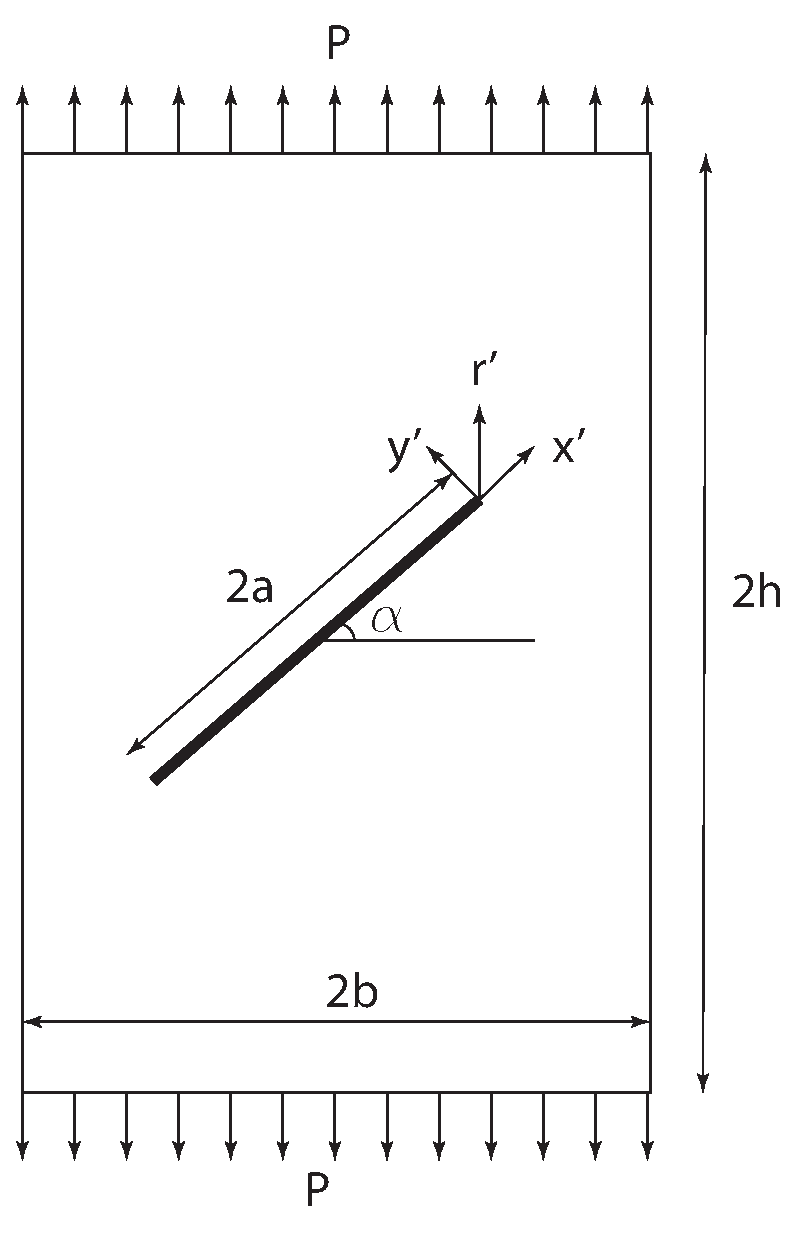
\includegraphics{isogeometric_sbfem/images/angled_crack_geo_bc.eps}
        }
        \caption{Angled crack in a rectangular orthotropic body: geometry}
        \label{iso_fig:angled_crack_geo_bc}
    \end{figure}

\paragraph{}
The elastic properties of the material are $E_{11} = E_{22}= E_{33}=15.4\times 10^6 psi$, $G_{12} = G_{23} = G_{13} = 15.7 \times 10^6 psi$, and $\nu_{12} = \nu_{23} = \nu_{13} = 0.4009$.
The results are compared with those obtained in \cite{Banks2005}.
The convergence of mode I and mode II SIF with mesh size is shown in tab.~\ref{iso_tab:angled_crack_convergence} for a crack at an angle $\alpha = \pi/12$.
The influence of the order of the shape functions is also shown.
It can be seen that increasing the number of degrees of freedom, the error in the numerical SIF decreases.
A very good agreement is observed.
\begin{table}
\caption{Convergence of the generalized stress intensity factors $
    (\mean{K_\RN{1}}, \mean{K_\RN{2}}) =
    (K_I,K_{II}) /
    P\sqrt(\pi a)
    $}
\label{iso_tab:angled_crack_convergence}
\begin{tabularx}{\textwidth}{XXXXX}
    \toprule
    \multirow{2}{*}{Order}& & \multicolumn{3}{c}{Number of DOF} \\
    \cmidrule{3-5}
    & & 160 & 240 & 320 \\
    \multirow{2}{*}{$2$}    &   $\mean{K_\RN{1}}$   &   1.2770  &   1.2723  &   1.2706  \\
                            &   $\mean{K_\RN{2}}$   &   0.2918  &   0.2915  &   0.2913  \\
    \multirow{2}{*}{$4$}    &   $\mean{K_\RN{1}}$   &   1.2700  &   1.2697  &   1.2697  \\
                            &   $\mean{K_\RN{2}}$   &   0.2914  &   0.2913  &   0.2913  \\
    \multirow{2}{*}{$6$}    &   $\mean{K_\RN{1}}$   &           &   1.2668  &   1.2670  \\
                            &   $\mean{K_\RN{2}}$   &           &   0.2913  &   0.2913  \\                           
    \midrule
    \bottomrule
\end{tabularx}
\end{table}

\paragraph{}
Also, increasing the order of the NURBS basis functions, the error decreases.
The influence of the crack orientation α on the mode \RN{1} and mode \RN{2} SIF is shown in tab.~\ref{iso_tab:angled_crack_sif_1} and tab.~\ref{iso_tab:angled_crack_sif_2}.
A total of 80 control points are used with different order of the NURBS basis functions.
It can be seen that a very good agreement is observed.
\begin{table}
\caption{Generalized stress intensity factors $K_\RN{1}/P\sqrt{\pi a}$ of angled crack in rectangular orthotropic body}
\label{iso_tab:angled_crack_sif_1}
\begin{tabularx}{\textwidth}{XXXXX}
    \toprule
    Angle   &   $K_\RN{1}$  &   \multicolumn{3}{c}{ }  \\
    \cmidrule{2-5} 
    $\alpha$&\cite{Banks2005}&  \multicolumn{3}{c}{Order of the curve}  \\
    \cmidrule{3-5} 
    & & 2 & 4 & 6 \\
    \midrule
    0         & 1.3755 & 1.3603 & 1.3583 & 1.3583 \\
    $\pi/12 $ & 1.2692 & 1.2706 & 1.2697 & 1.2670 \\
    $\pi/ 6 $ & 1.0268 & 1.0277 & 1.0270 & 1.0270 \\
    $\pi/ 4 $ & 0.6952 & 0.6941 & 0.6944 & 0.6943 \\
    $\pi /3 $ & 0.3579 & 0.3582 & 0.3580 & 0.3580 \\
    $5\pi/12$ & 0.1095 & 0.0996 & 0.1003 & 0.1004 \\
    \bottomrule
\end{tabularx}
\end{table}

\begin{table}
    \caption{Generalized stress intensity factors $K_\RN{2}/P\sqrt{\pi a}$ of angled crack in rectangular orthotropic body}
    \label{iso_tab:angled_crack_sif_2}
    \begin{tabularx}{\textwidth}{XXXXX}
        \toprule
        Angle   &   $K_\RN{2}$  &   \multicolumn{3}{c}{ }\\
        \cmidrule{2-5}
        $\alpha$&\cite{Banks2005}&  \multicolumn{3}{c}{Order of the curve}\\
        \cmidrule{3-5}
        & & 2 & 4 & 6 \\
        \midrule
        0         & 0.0000 & 0.0000 & 0.0000 & 0.0000 \\
        $\pi/12 $ & 0.2912 & 0.2914 & 0.2913 & 0.2913 \\
        $\pi/ 6 $ & 0.5092 & 0.5087 & 0.5093 & 0.5092 \\
        $\pi/ 4 $ & 0.5807 & 0.5948 & 0.5946 & 0.5946 \\
        $\pi /3 $ & 0.5248 & 0.5247 & 0.5248 & 0.5248 \\
        $5\pi/12$ & 0.3108 & 0.3119 & 0.3117 & 0.3117 \\
        \bottomrule
    \end{tabularx}
\end{table}

\pagebreak